\subsection{\name{} Runtime}\label{sec:runtime}

% \begin{figure}[t!]
% 	\centering
% 	\scalebox{1}{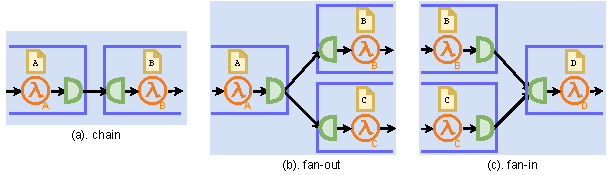
\includegraphics[width=\columnwidth]{figures/deorc-patterns.pdf}}
% 	\caption{\deorc{} implements transitions in a decentralized manner where
% the egress on the source function(s) and ingress on the target function(s)
% work together to execute the orchestration. \shadi{does this figure add value given you have Fig 1. you can probably combine the patterns there ans name them there and reuse that figure.}}
% 	\label{fig:transition}
% \end{figure}

\begin{figure}[]
    \begin{minted}[
    frame=single,
    fontsize=\scriptsize
  ]{json}
{
    "Data": {
        "Source": "http | dynamodb | s3 | ...",
        "Value": "<object> | [<pointers>]"
    },
    "Session": "uuid",
    "Fan-out": {
        "Index": "int",
        "Size": "int",
        "OuterLoop": {
            "Index": "int",
            "Size": "int"
        }
    }
}
    \end{minted}
    \caption{\name{} runtime input payload schema}
    \label{fig:input-format}
\end{figure}


In this section, we describe how \name{} efficiently implements orchestration
and the six transition patterns in a decentralized manner. \name{} adds a
runtime library to each  user function to perform the transitions. The \name{}
runtime consists of an ingress and an egress component. During execution, the
egress on the source function(s) and ingress on the target function(s) work
together to execute the transition. The egress interprets its \name{}
configuration to learn what transition it needs to perform. The ingress reads
and formats input data sent by egress so that
\name{} orchestration logic can happen transparently without any change to the
user code.

A key requirement of \name{}'s design is to only use the basic serverless
abstraction without relying on any specialized APIs. Therefore, we build the
runtime such that it only depends on two serverless components that are
universally supported by all platforms: i.
asynchronous invocation of FaaS functions (e.g., as available in AWS Lambda, Azure Functions,
Google Cloud Funtions, Openwhisk) and ii. a strongly consistent data store
that supports conditional write operations (e.g., DynamoDB, Cosmos DB).

We describe how the \name{} runtime uses the two basic abstraction to support
each workflow pattern below:

\noindent\textbf{chain} 
The chain pattern involves one egress on source function and one ingress on
the target function. The source egress simply invokes the target function with
the source function's user code's output. \name{} uses asynchronous invocation
to avoid waiting and idle-billing.

When the target function is invoked, the input is first received by the
\name{} ingress. The ingress uses read the user function's input data, either
directly from the input payload or from a data store (e.g., if the
asynchronous invocation is via a storage trigger). Finally, ingress calls its
user function and passes it the input.

\noindent\textbf{fan-out}
The fan-out pattern involves one egress on the source function and many
ingresses on the target functions.
Similar to chaining, the egress asynchronously invokes each target and the
ingresses on targets read the input data sent from the source and passes it to
its user function.

\noindent\textbf{map}
map is a simple variation of fan-out where the egress treats its user code
output as an iterable. For each element in the iterable, the source egress
invokes the same target function to launch a unique runtime instances and pass
it the element.

\noindent\textbf{branch}
Branch is similar to fan-out except that each branch has a condition attached
and only executes when the condition evaluates to true. The egress first
evaluates the boolean condition before invoke the target function in that
branch. \shadi{is branch similar to fan-out or chain?}

\textbf{fan-in}
The fan-in pattern involves one ingress node and many egress nodes.
It is the main complexity of decentralized orchestration as we want to ensure
that the transition is \emph{wait-free} to avoid idle-billing. In particular,
we want to invoke the sink function only when all upstream functions have
completed so that the sink function does not have to be spun up ahead of time and
wait for upstream functions to finish. Moreover, the upstream functions should
simply terminate when done instead of waiting for each other.

To achieve this, \name{} relies on a strongly consistent data store with
conditional writes. \name{} egress always writes the output of the fan-in
source functions to an intermediary data store. The write not only signals the
completion of a function, but also allows any of the source functions in a
fan-in to access the output of each other. This way, each egress can simply
write its output and terminate, and the last-to-finish source function will
invoke the sink function.
\name{} requires this data store to be ``strongly consistent''. This is needed
to prevent the scenarios where all egress have written outputs but none of
them sees that all have completed, which results in the sink function never
invoked.

Additionally, fan-in makes sure that the sink function is only invoked once.
\name{} achieves this by having the egress nodes synchronize with each other
via intermediary data store such that only the last-to-finish egress invokes
the sink function. Synchronization is done with atomic read-after-write over a
single object, which requires the conditional write ability from the data
store. Specific implementation depends on the data store and we discuss the
details in \S\ref{sec:impl}.

The last-to-finish egress invokes the sink function with a vector of pointers
to each upstream function's stored output. The pointers are the in same order
as the vector of upstream function names. The ingress on the sink function
dereferences each point by reading from the data store and passes a vector of
output values to its user function.


\subsubsection{Runtime Metadata}

To support a rich variety of orchestration patterns, \name{} requires a
specific input payload schema in JSON (Figure~\ref{fig:input-format}) that
contains \name{} runtime metadata. In particular, \name{} uses the
\texttt{Fan-out} field to store branch indexes. The \texttt{Fan-out} field
contains a recursive \texttt{OuterLoop} field that supports nested fan-outs.

The runtime additionally uses a \texttt{Session} field to support concurrent
invocations of the same workflow. The \texttt{Session} field is a UUID string
that is unique to a workflow invocation and shared by all constituent function
instances in the invocation. Function checkpoint names are prefixed by the \texttt{Session} string so that
concurrently invocations do not overwrite each other's data. We discuss the details on
\name{} checkpoints and execution guarantees in the Section~\ref{sec:exec-gntee}.